\documentclass{beamer}
\usepackage[utf8]{inputenc}
\usetheme{Madrid}
\usecolortheme{default}
\usepackage{amsmath,amssymb,amsfonts,amsthm}
\usepackage{txfonts}
\usepackage{tkz-euclide}
\usepackage{listings}
\usepackage{adjustbox}
\usepackage{array}
\usepackage{tabularx}
\usepackage{gvv}
\usepackage{lmodern}
\usepackage{circuitikz}
\usepackage{tikz}
\usepackage{graphicx}

\setbeamertemplate{page number in head/foot}[totalframenumber]

\usepackage{tcolorbox}
\tcbuselibrary{minted,breakable,xparse,skins}



\definecolor{bg}{gray}{0.95}
\DeclareTCBListing{mintedbox}{O{}m!O{}}{%
  breakable=true,
  listing engine=minted,
  listing only,
  minted language=#2,
  minted style=default,
  minted options={%
    linenos,
    gobble=0,
    breaklines=true,
    breakafter=,,
    fontsize=\small,
    numbersep=8pt,
    #1},
  boxsep=0pt,
  left skip=0pt,
  right skip=0pt,
  left=25pt,
  right=0pt,
  top=3pt,
  bottom=3pt,
  arc=5pt,
  leftrule=0pt,
  rightrule=0pt,
  bottomrule=2pt,
  toprule=2pt,
  colback=bg,
  colframe=orange!70,
  enhanced,
  overlay={%
    \begin{tcbclipinterior}
    \fill[orange!20!white] (frame.south west) rectangle ([xshift=20pt]frame.north west);
    \end{tcbclipinterior}},
  #3,
}
\lstset{
    language=C,
    basicstyle=\ttfamily\small,
    keywordstyle=\color{blue},
    stringstyle=\color{orange},
    commentstyle=\color{green!60!black},
    numbers=left,
    numberstyle=\tiny\color{gray},
    breaklines=true,
    showstringspaces=false,
}
%------------------------------------------------------------
%This block of code defines the information to appear in the
%Title page
\title %optional
{2.2.19}

%\subtitle{A short story}

\author % (optional)
{RATHLAVATH JEEVAN -AI25BTECH11026}



\begin{document}


\frame{\titlepage}
\begin{frame}{Question}
The scalar product of the vector $\hat{i} + \hat{j} + \hat{k}$ with a unit vector along the sum of vectors 
$2\hat{i} + 4\hat{j} - 5\hat{k} \quad \text{and} \quad \lambda \hat{i} + 2\hat{j} + 3\hat{k}$ is equal to one. Find the value of $\lambda$.
 
\end{frame}
\begin{frame}{Theoretical Solution}

\textbf{Solution:}\\
 \textbf{Given:}  
\begin{align}
\vec u = \myvec{1\\1\\1}, \quad 
\vec a = \myvec{2\\4\\-5}, \quad 
\vec b = \myvec{\lambda\\2\\3}
\end{align}
We require:  
\begin{align}
\vec u^\top \frac{\vec a+\vec b}{\|\vec a+\vec b\|} = 1
\end{align}

\textbf{Sum of vectors:}
\begin{align}
\vec a + \vec b = \myvec{2+\lambda\\6\\-2}
\end{align}
\end{frame}

\begin{frame}{Theoretical Solution}
\textbf{Dot product:}
\begin{align}
\vec u^\top(\vec a+\vec b) = \myvec{1 & 1 & 1}\myvec{2+\lambda\\6\\-2} 
= (2+\lambda)+6+(-2) = \lambda+6
\end{align}

\textbf{Norm of the sum:}
\begin{align}
\|\vec a+\vec b\| = \sqrt{(2+\lambda)^2+6^2+(-2)^2}
= \sqrt{(2+\lambda)^2+40}
\end{align}
 \textbf{Condition:}
 
\begin{align}
\frac{\lambda+6}{\sqrt{(2+\lambda)^2+40}} = 1
\end{align}
\end{frame}
\begin{frame}{Theoretical Solution}
\textbf{Simplify:}
\begin{align}
\lambda+6 = \sqrt{(\lambda+2)^2+40}
\end{align}
Squaring,
\begin{align}
(\lambda+6)^2 = (\lambda+2)^2+40
\end{align}
\begin{align}
\lambda^2+12\lambda+36 = \lambda^2+4\lambda+44
\end{align}
\begin{align}
8\lambda = 8 \quad \Rightarrow \quad \lambda = 1
\end{align}
\textbf{Conclusion:}  
The required value is
\begin{align}
\boxed{\lambda=1}
\end{align}
\begin{align}
\boxed{\,a = -3\,}
\end{align}

\end{frame}

\begin{frame}[fragile]
    \frametitle{C Code}
    \begin{lstlisting}
#include <stdio.h>
#include <math.h>

int main() {
    double lambda1, lambda2;

    // Equation: (lambda + 6) / sqrt((lambda+2)^2 + 40) = 1
    // Square both sides => (lambda+6)^2 = (lambda+2)^2 + 40

    // Expanding manually:
    // lambda^2 + 12lambda + 36 = lambda^2 + 4lambda + 44
    // => 8lambda = 8
    // => lambda = 1

    lambda1 = 1;
     \end{lstlisting}
\end{frame}
\begin{frame}[fragile]
    \frametitle{C Code }
    \begin{lstlisting}
    printf("The value of lambda is: %.2f\n", lambda1);

    return 0;
}

    \end{lstlisting}
\end{frame}
\begin{frame}[fragile]
    \frametitle{Python Code}
    \begin{lstlisting}
import numpy as np
import matplotlib.pyplot as plt
from mpl_toolkits.mplot3d import Axes3D

# Vectors
v1 = np.array([2, 4, -5])
v2 = np.array([1, 2, 3])  # lambdai + 2j + 3k

# lambda = 1 solution
lam = 1
v_sum = np.array([2+lam, 6, -2])

# Vector (i + j + k)
u = np.array([1, 1, 1])

# Create A4 figure (8.27 * 11.7 inches)
fig = plt.figure(figsize=(8.27, 11.7))
ax = fig.add_subplot(111, projection='3d')
    \end{lstlisting}
\end{frame}

\begin{frame}[fragile]
    \frametitle{Python Code}
    \begin{lstlisting}
# Plot vectors
ax.quiver(0, 0, 0, v1[0], v1[1], v1[2], color='r', label='2i+4j-5k')
ax.quiver(0, 0, 0, lam*v2[0], lam*v2[1], lam*v2[2], color='b', label='lambdai+2j+3k (lambda=1)')
ax.quiver(0, 0, 0, v_sum[0], v_sum[1], v_sum[2], color='g', label='Sum vector')
ax.quiver(0, 0, 0, u[0], u[1], u[2], color='m', label='i+j+k')

# Labels and title
ax.set_xlabel('X axis')
ax.set_ylabel('Y axis')
ax.set_zlabel('Z axis')
ax.set_title('3D Graph of Vectors (lambda=1)', fontsize=14)
ax.legend()
    \end{lstlisting}
\end{frame}

\begin{frame}[fragile]
    \frametitle{Python Code}
    \begin{lstlisting}
# Save as A4 size PDF and PNG
plt.savefig("vector_solution_lambda_A4.png", dpi=300, bbox_inches='tight')
plt.savefig("vector_solution_lambda_A4.pdf", bbox_inches='tight')

plt.show()

print("Saved as vector_solution_lambda_A4.png and vector_solution_lambda_A4.pdf")
    \end{lstlisting}
\end{frame}

\begin{frame}{Plot}
    \centering
    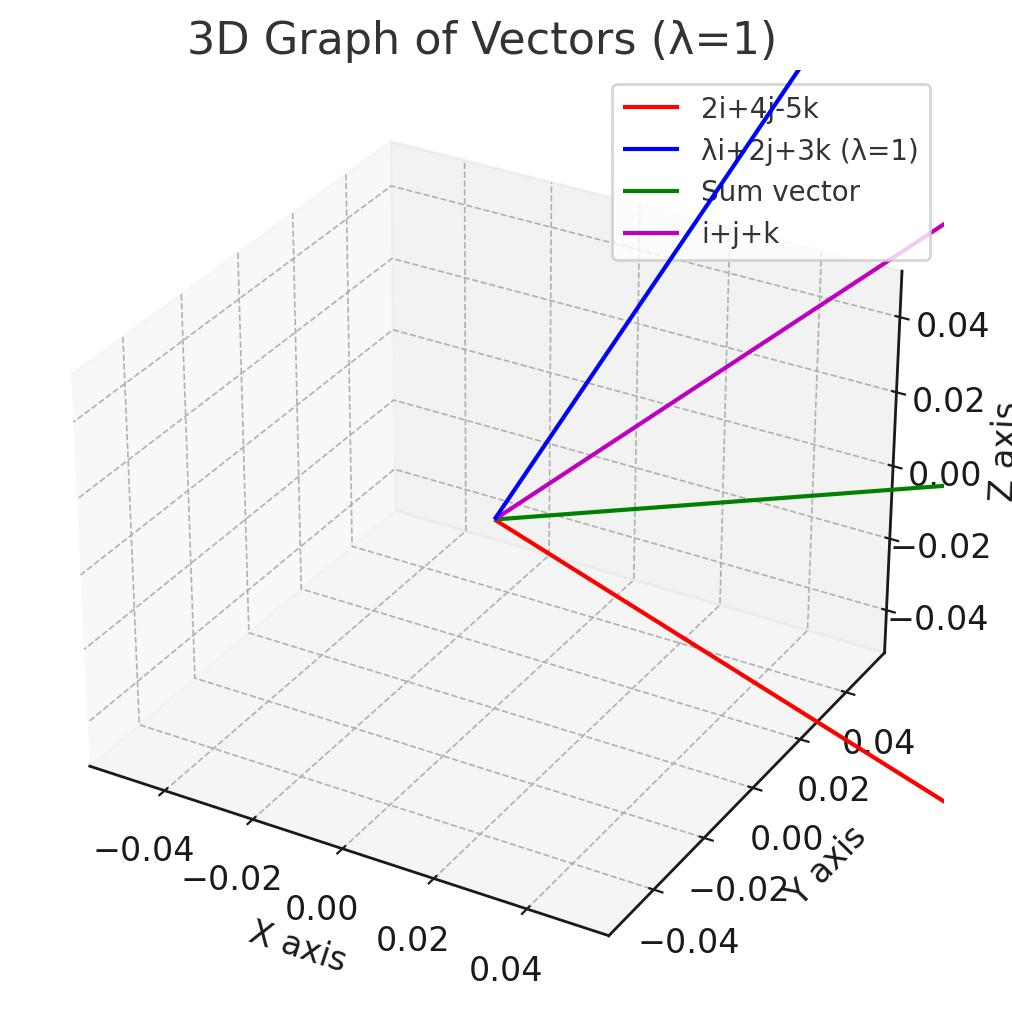
\includegraphics[width=\columnwidth, height=0.8\textheight, keepaspectratio]{beamer/figs/matg3.jpeg}     
\end{frame}




\end{document}